% !TEX root = thesis.tex

\chapter{Simulation results}
\label{ch:sim_results}

\section{Introduction}


\begin{sidewaystable}
 \centering
 \footnotesize
 \begin{tabular}{lx{0.8cm}x{1.4cm}x{0.7cm}x{1cm}x{0.8cm}x{0.8cm}x{0.7cm}x{1.9cm}}
\toprule
name & peric. \newline (kpc) & $\log_{10}$(M$_\star$) \newline (M$_\odot$) & $R_e$ \newline (kpc) & $\sigma_\star$ \newline (km/s) & M$_V$ \newline (mag) & M$_{r'}$ \newline (mag) & $n$ & $\bar{\mu}_{e,r'}$ \newline (mag/arcsec$^2$) \\
\midrule
  62 &                        50 &                                        6.50 &                  1.6 &                            6.7 &                 -9.7 &                   -10.1 & 1.1 &                                         28.7 \\
  62 &                       100 &                                        6.57 &                  1.6 &                            8.0 &                 -9.9 &                   -10.2 & 1.0 &                                         28.5 \\
  62 &                       150 &                                        6.59 &                  1.6 &                            9.1 &                 -9.9 &                   -10.2 & 1.4 &                                         28.6 \\
  62 &                       200 &                                        6.59 &                  1.7 &                            8.3 &                -10.0 &                   -10.3 & 1.2 &                                         28.5 \\
  62 &                       300 &                                        6.64 &                  1.7 &                            8.6 &                -10.1 &                   -10.4 & 1.0 &                                         28.2 \\
  71 &                        50 &                                        6.26 &                  6.7 &                           21.6 &                 -9.5 &                    -9.8 & 0.0 &                                         31.8 \\
  71 &                       100 &                                        6.82 &                  6.2 &                            6.5 &                -10.9 &                   -11.2 & 0.5 &                                         30.5 \\
  71 &                       150 &                                        6.79 &                  6.4 &                            0.8 &                -10.7 &                   -11.0 & 0.5 &                                         30.5 \\
  71 &                       200 &                                        6.85 &                  6.9 &                            0.8 &                -11.0 &                   -11.3 & 0.2 &                                         30.4 \\
  71 &                       300 &                                        6.85 &                  7.2 &                            1.8 &                -11.0 &                   -11.4 & 0.2 &                                         29.7 \\
  69 &                        50 &                                        6.81 &                  7.6 &                            1.6 &                -10.6 &                   -11.0 & 0.2 &                                         30.7 \\
  69 &                       100 &                                        7.53 &                  7.1 &                           17.8 &                -12.5 &                   -12.9 & 0.1 &                                         28.4 \\
  69 &                       150 &                                        8.05 &                  4.3 &                           11.6 &                -14.2 &                   -14.4 & 0.3 &                                         26.8 \\
  69 &                       200 &                                        8.34 &                  3.3 &                           18.4 &                -15.0 &                   -15.3 & 1.0 &                                         25.0 \\
  69 &                       300 &                                        8.42 &                  1.8 &                           23.9 &                -15.5 &                   -15.7 & 0.9 &                                         23.5 \\
  68 &                        50 &                                        6.27 &                  8.0 &                            nan &                 -9.1 &                    -9.4 & 0.0 &                                         32.3 \\
  68 &                       100 &                                        6.85 &                  7.3 &                            2.5 &                -10.6 &                   -10.9 & 0.1 &                                         31.2 \\
  68 &                       150 &                                        6.85 &                  7.3 &                            nan &                -10.6 &                   -10.9 & 0.1 &                                         31.2 \\
  68 &                       200 &                                        7.02 &                  7.4 &                            nan &                -11.4 &                   -11.7 & 0.1 &                                         30.0 \\
  68 &                       300 &                                        8.09 &                  3.8 &                           11.5 &                -14.5 &                   -14.8 & 0.8 &                                         26.2 \\
  41 &                        50 &                                        8.93 &                  3.5 &                           16.5 &                -16.2 &                   -16.5 & 1.0 &                                         23.9 \\
  41 &                       100 &                                        8.94 &                  2.5 &                           26.0 &                -16.4 &                   -16.7 & 1.0 &                                         23.0 \\
  41 &                       150 &                                        8.99 &                  1.7 &                           28.5 &                -16.6 &                   -16.8 & 0.8 &                                         22.2 \\
  41 &                       200 &                                        8.97 &                  2.2 &                           29.4 &                -16.6 &                   -16.8 & 0.8 &                                         22.5 \\
  41 &                       300 &                                        9.04 &                  1.8 &                           33.7 &                -17.0 &                   -17.2 & 0.7 &                                         21.8 \\
\bottomrule
\end{tabular}

 \caption{Features of the selected MoRIA galaxies at $z=0$.} \label{tbl:galaxies}
\end{sidewaystable}


\paragraph*{Radial period}
Pericenter passages, as explained in the following, are important moments for the life of the simulated dwarf.
In order to compare different orbits, we normalise the simulation time by the orbital radial period $T_r$, i.e. the time between two pericenter passages, \citep[p.~146]{BinneyTremaine2008}:
\begin{equation}
    T_r = 2 \int^{r_a}_{r_p} \frac{\d r}{\sqrt{2\left[E-\Phi(r) \right] - J^2/r^2}}
    \label{eq:radial_period}
\end{equation}
where $r_p, r_a$ are the pericenter and apocenter distance respectively, $E$ and $J$ the orbital energy and angular momentum per unit mass, $\Phi(r)$ the potential at radius $r$ of the NFW halo around which the galaxy is orbiting.

By defining the time of pericenter passage as $t_p: r(t_p) = r_p$, we can introduce the normalized time:
\begin{equation}
\tau = \frac{t-t_p}{T_r},
\end{equation}
which is~$0$ or $1$ for first or second pericenters respectively,~and~$0.5$ for apocenter passages.

% We begin with following one galaxy in its journey around the cluster.
In the following we will compare the effects of orbit and initial mass using the set of 25 simulations we have carried out.


\paragraph*{Tidal radius}
As we shall see, the cluster gravitational potential is able to strip material from the galaxy. Some of the simulations, depending on the orbit they are on, will become gravitationally unbound dominated by the cluster potential.
We chose to define the event of becoming unbound using the condition on the tidal radius \cite{King1962}: namely when it becomes smaller than the effective radius.
This criterion tests whether the stellar body of the galaxy will be dissolved or not which is the criterion on which an observer would base the detection of a "galaxy''.
Physically, also this implies that orbits of the stars in the outskirts of the galaxy are influenced by the cluster potential more than they are by the galactic halo potential. 
Tidal radius $r_t$ is computed as following.
\begin{equation}
r_t = r \sqrt[3]{\frac{M_g}{M_c(r) (3+e)}}
\label{eq:tidal_radius}
\end{equation}
where $e = (r_a - r_p) / (r_a + r_p)$ is the eccentricity of the orbit computed, $r_a$, $r_p$ the apocenter and pericenter radii respectively; $M_c(r)$ is the enclosed cluster mass at radius $r$, and $M_g$ the instantaneous total mass of the galaxy.
As a convention we measure the galaxy mass as the total mass (baryonic and dark matter) within $10$~kpc from the center of the galaxy.

In Figure \ref{fig:tidal_radius} we show an example of $r_t$ evolution along the orbit.
We define a galaxy to become unbound when the condition 
\begin{equation}
    R_e > r_t
\label{eq:tidal_radius_condition}
\end{equation}
first occurs.
%Galaxies on a radial orbits will undergo disruption more easily.
\begin{figure}
\centering
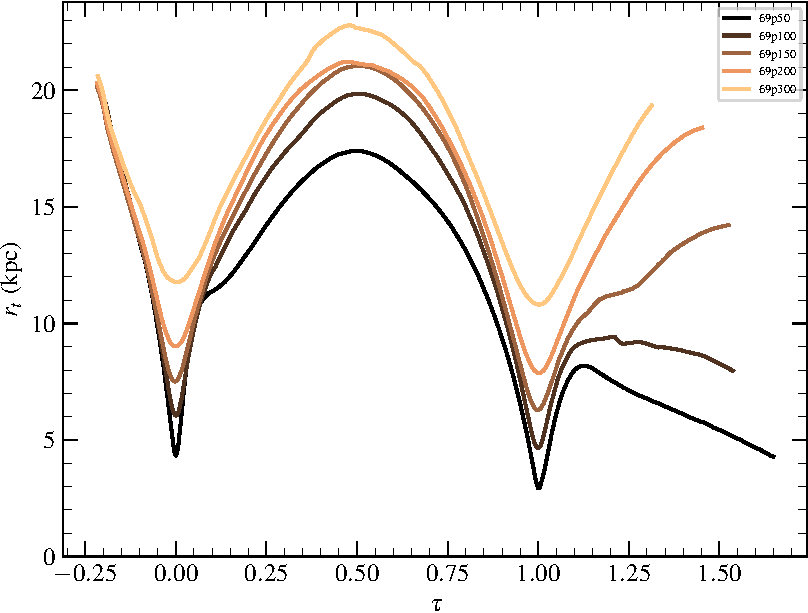
\includegraphics[width=\textwidth]{14.0_tidal_radius.pdf}
\caption{Evolution of the tidal radius for the simulations ID 69.}
\label{fig:tidal_radius}
\end{figure}

\section{Becoming an Ultra Diffuse Galaxy (UDG)}
\label{sec:UDG}

Faint Low Surface Brightness (LSB) galaxies with $R_e > 1$ kpc have been detected in galaxy clusters since the 1980s \citep[e.g.][]{Sandage1984}.
% See Wittmann  https://www2.mpia-hd.mpg.de/homes/galClusters_2017/slides/Ringberg2017_presentation_Wittmann.pdf

% Wittmann2017 studies LSB in Perseus
LSB galaxies are defined as having \citep{Venhola2017}:
\begin{equation}
\begin{cases}
 \mu_{0,r'} > 23 \mbox{ mag/arcsec}^2\\
 M_{r'} > -19
\end{cases}
\end{equation}

In 2015 \citet{VanDokkum2015} introduced a size criterion to distinguish between more compact 'normal' dwarfs \citep{Sales2021}:
UDG are therefore defined as large ($R_e > 1.5$~kpc) low surface brightness galaxies.
%($\bar\mu_{r',e} > 24$~mag/arcsec$^2$).

The majority of studies indicate that they have the properties of large dwarf galaxies \citep{Sandage1984, Roman2017, Venhola2017, Saifollahi2021}.
Three main mechanisms are hypothesised as possible formation scenarios for UDGs \citep{Rong2020}:
dwarf galaxies which undergo strong tidal stripping \citep{Venhola2017, Carleton2018, Rong2020a},
gas outflows driven by stellar feedback with extended dark matter halo and faint and diffuse stellar component \citep{DiCintio2017, ManceraPina2019},
or failed $L_\star$ galaxies\footnote{with $L_\star$ galaxies it is meant a galaxy with luminosity around the characteristic luminosity scale in the Schechter luminosity function \citep{Press1974}, and it can be approximated to be $L_\star \approx 3\times10^{11}L_\odot$, \cf{}  \citet{Cooray2005}.} in high mass dark halos with ceased star formation in the early universe.

Some UDGs have earlier been identified as disrupted early-type galaxies.
\citet{Koch2012} is indeed able to reproduce a typical S-shape tidal tailed UDGs HCC-087 in the Hydra I cluster. 
In the Coma and Abell 1314 clusters \citep{Yagi2016, ManceraPina2019} UDGs are preferably aligned towards the cluster center.

In the Fornax cluster, the low statistics do not allow for a conclusive analysis.
On the other hand at least two of the detected UDGs show sign of elongation towards a nearby dwarf galaxy \citep[with $M_{r'} > -19$~mag, see][]{Venhola2017}.

\paragraph{UDGs in Fornax}
\citet{Venhola2017} found nine UDGs candidates within an area of 4~deg$^2$ centered in NGC1399.
The relative number of UDGs w.r.t. dwarf galaxies in Fornax is consistent with the same value in the Coma and Virgo clusters.
Also, the number of UDGs within the virial radius are correlated with the virial mass of the cluster.
In the size-magnitude parameter space, UDGs in Coma form a continuous distribution, whereas in Fornax two of them are  remarkably luminous, and can be considered as outliers.
Also, UDGs in Fornax are among the more luminous galaxies and their colour correlates with surface brightness, becoming redder with increasing surface brightness.
They follow the same color-magnitude relation as dwarfs, which suggests a link between UDGs and dwarf galaxies  (\cf{} Section~\ref{sec:CM}).
% As expected, Sérsic index is around $1$ 
As opposed to the ones in the Coma cluster, their alignment w.r.t. the cluster potential is not evident: in Coma UDGs are oriented towards the cluster center, whereas in Fornax, as mentioned above, there's no correlation.
It is interesting to note that larger UDGs are more elongated as opposed to UDGs in Coma.

\subsection{Size and magnitudes}
According to the virial theorem %predicts that by adding energy to a galaxy, it will increase its radius: 
once approaching the pericenter, energy is transferred to the galaxy: stars thus migrate to more energetic and hence wider orbits.
In addition, mass is lost due to tides, making the gravitational well even more shallow and leading to potentially large increases in radius.
We compute the 3D effective radius shown in Figure~\ref{fig:r_eff}.
This radius is independent of the orientation of the galaxy, and it has been computed as the radius of the sphere which contains half the total luminosity of the galaxy.
Tidal heating affects the size of the galaxies as they pass near the cluster center, with low mass galaxies affected most.

% We compare the resulting effective radius in simulations with the ones not taking into account the gas inside the cluster, Figure~\ref{fig:r_eff_no_gas}.

\begin{figure}[ht]
\centering
\includegraphics[width=\textwidth]{{00.0_fig_3dreff_time}.pdf}
\caption{3d effective radius evolution with time normalised with the radial period of the orbit. Curves are smoothed using a rolling average of 0.2~Gyr and are truncated as soon as condition \eqref{eq:tidal_radius_condition} is verified.}
\label{fig:r_eff}
\end{figure}

% FIXME See whether to put this plot
% \begin{figure}
% \centering
% \includegraphics[width=\columnwidth]{{00.2_3dreff_gas_no_gas_last_Re_color}.pdf}
% \caption{Relative change in effective radius between simulations with tides only ($R^{3D}_{e, ng}$), and cluster infall simulations with RPS ($R^{3D}_e$) at redshift $z=0$.}
% \label{fig:r_eff_no_gas}
% \end{figure}
% \subsection{Dark halo concentration}
% Between two pericenters material falls back in the galaxy, see Figure~\ref{fig:dm_halo}.

% TODO maybe it is better to compare a sphere of 2 kpc with one of 10 kpc, and not comparing spheres with cubes.

% \begin{figure}
% \centering
% \includegraphics[width=0.9\columnwidth]{{12.0_dm_ratio}.pdf}
% \caption{Ratio between dark matter mass contained in a sphere of $10$ kpc radius $M_h^{c}$ and the total dark matter mass contained in the moving box, $M_h^{tot}$.}
% \label{fig:dm_halo}
% \end{figure}

% \subsection{Stellar metallicity gradients}

\subsection{$M_h/M_\star$}
We computed the amount of stellar and dark matter mass inside a sphere of radius $10$~kpc centered on the dwarf and the masses inside the entire moving box.
While stars gets formed around pericenter passages, dark matter instead is pulled out by tidal forces who elongate the halo, effectively stripping dark matter particles out of the moving box of our simulation setup.
This is confirmed for example by comparing the amount of dark matter inside the $10$~kpc region around the dwarf with the whole dark matter present inside the moving box.
As shown in Figure \ref{fig:dm_center_inflow}, there is an inflow of dark matter towards the dwarf galaxy due to tidal squeezing and compression, soon followed by an expansion, resulting in a dearth of dark matter after the first pericenter passage. % TODO dark matter profile around pericenter?
For very radial orbits, around first infall, central halo mass increases more than the stellar mass created by the starburst, Figure~\ref{fig:m_halo_m_star}.

% TODO This is linked to the velocity dispersion which is essentially tracing the amount of mass loss.

\begin{figure}
\centering
\includegraphics{{12.5_dm_ratio_one_sim}.pdf}
\caption{Relative amount of central dark matter $M_{h}^c$
(computed as the mass inside a sphere of 10~kpc of radius around the galaxy)
w.r.t. the dark matter in the simulation box ($M_{h}^{tot}$) for sim ID 69.
Colours indicate the pericenter distances of the different orbits.
}
\label{fig:dm_center_inflow}
\end{figure}
\begin{figure}
\centering
\includegraphics[height=0.95\textheight]{{12.1_m_halo_m_star}.pdf}
% \includegraphics[width=0.75\columnwidth]{{12.1_m_halo_m_star}.pdf}
\caption{$M_h/M_\star$ around first infall. Halo and stellar mass are computed in the $10$~kpc sphere around the galaxy.
The different orbits with the respective pericenters are color coded and shown in the legend.}
\label{fig:m_halo_m_star}
\end{figure}

\subsection{Central stellar velocity dispersion}
We measured the central (within $250$ pc) stellar velocity dispersion for all the simulations on their orbits, as shown in Figure~\ref{fig:sigma}.
\begin{figure}[ht]
\centering
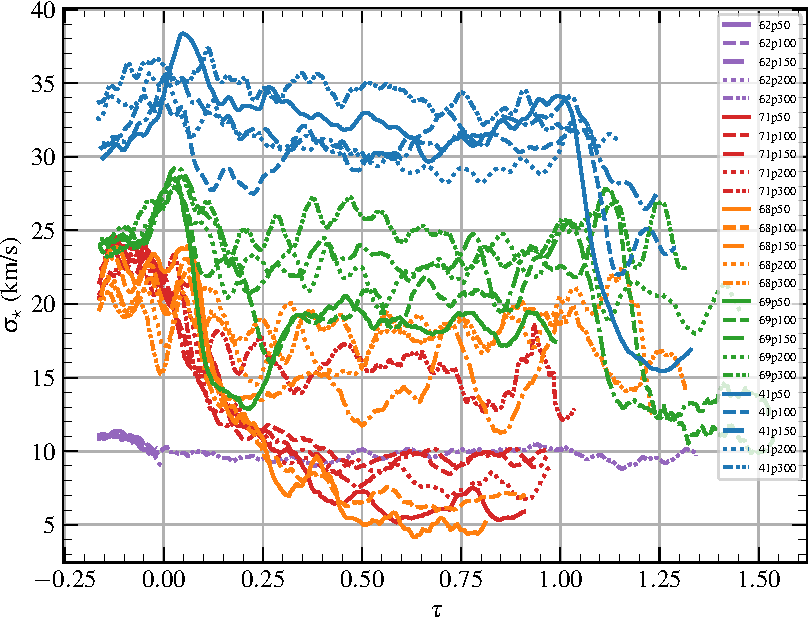
\includegraphics[width=\textwidth]{01.0_fig_sigma_time.pdf}
\caption{Velocity dispersion evolution as a function of time normalised with the radial period of the orbit.
}
\label{fig:sigma}
\end{figure}
For simplicity we adopted a common point of view for all the orbits, and the line-of-sight velocity dispersion is computed assuming the observer laying on the orbital plane.
As tidal interactions stir the particles in the center of the galaxies, at the pericenter passages a bump in the central velocity dispersion (denoted by~$\sigma$) can be seen.
The following temporary decrease in central velocity dispersion can be linked to the variations of~$M_h/M_\star$.
Tidal squeezing increase~$\sigma$ while subsequent mass loss can dramatically lower it.

We checked the dynamical mass estimation which can be computed from the velocity dispersion using the \citet{Wolf2010} relation:
\begin{equation}
\label{eq:wolf}
M^{dyn}_{est} = \dfrac{3}{G} \sigma_e^2 R_e,
\end{equation}
where $\sigma_e$ is the luminosity-weighted line-of-sight velocity dispersion within an effective radius~$R_e$,
and $G$ the gravitational constant.
The result for one simulation is shown in Figure~\ref{fig:wolf}.
The estimation with equation \eqref{eq:wolf} overestimates the mass by $\approx20-50\%$.
\begin{figure}[ht]
\centering
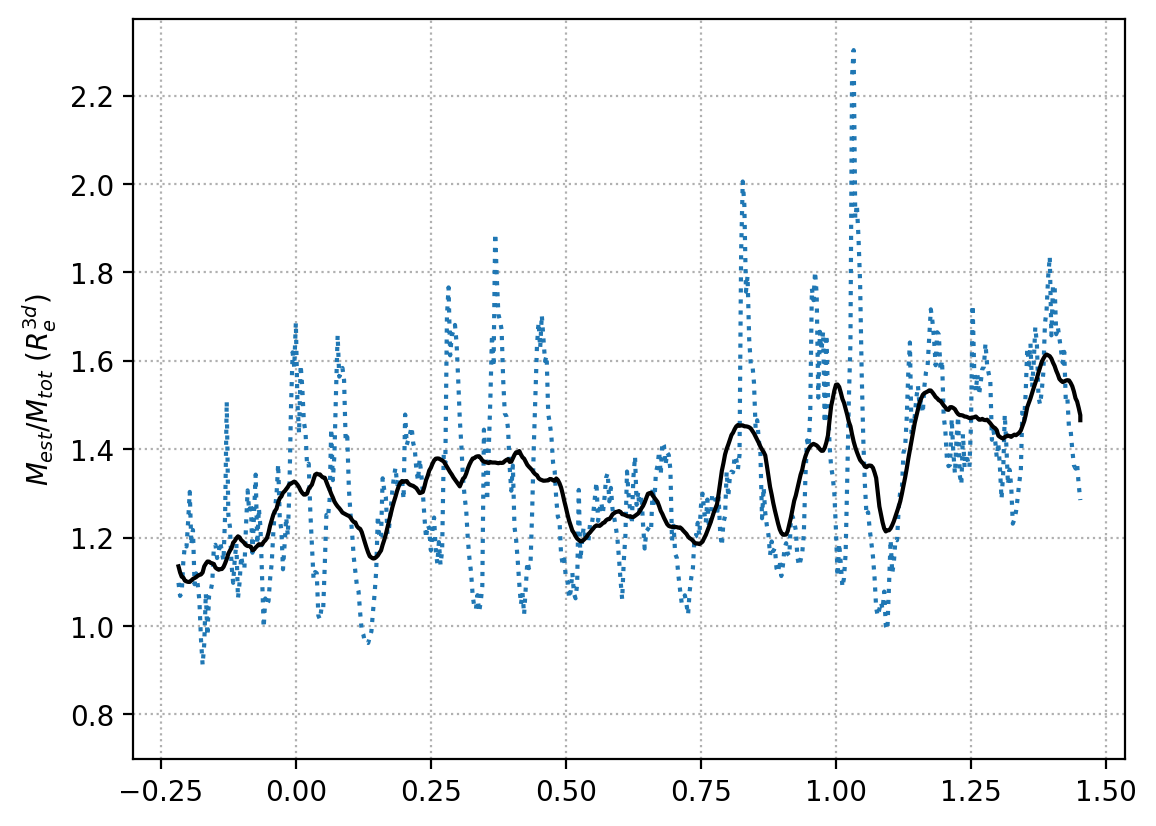
\includegraphics[width=\textwidth]{wolf_m_est_ratio69p200.png}
\caption{In blue the estimated mass from velocity dispersion with equation \eqref{eq:wolf} relative to the total mass within an effective radius computed from simulation particles,
for simulation ID 69 on an orbit with 200 kpc pericenter.
In black the local rolling average with a window of 30 snapshots.
}
\label{fig:wolf}
\end{figure}
%TODO The anisotropy parameter $\beta$ is shown

% \citep{Danieli2019} Low dark matter galaxies.

\subsection{3D ellipticity}
We computed the 3D ellipticity of the stellar component of the galaxies using the Principal Components Analysis (PCA).
The first principal component $\vect{w}_2$ is the direction of highest elongation (largest variance of the N star particle positions) computed via PCA\footnote{$\vect{w}_2$ is defined as the eigenvector corresponding to the largest eigenvalue of the covariance matrix $C = \frac 1 {(N-1)} AA^T$, where $A$ is the matrix of the position of the star particles centered on the barycenter of the stars.}.
% For now I took into account only the position of the star particles (which have negligible mass difference among them).

Around pericenter the main elongation direction of the ellipsoid ($\vect w_2$) is aligned with the cluster center; then it undergoes a ``slingshot effect" after pericenter and it aligns with the cluster center also around apocenter before falling back in. This behaviour is shown in Figure~\ref{fig:pca}.
Around the second pericenter passage, for radial orbits, the galaxy ends up being dispersed and not anymore gravitationally bound.

In Figure~\ref{fig:pca_angle_r}, we show quantitatively the relative orientation between $\vect{w}_2$ and the clustercentric direction for simulation ID 69.
Around both pericenter passages the galaxy becomes aligned with the cluster center.
The maximum alignment is obtained at a delayed time depending on the radiality of the orbit.
Also, for all the orbits, the galaxy shows an aligment of an angle $<30$~deg if the orbital phase lays within a quarter of the radial period from pericenter. % ($t \in t_p \pm 0.25 T_r$).
Except for the orbit with 100 kpc pericenter, it is possible to see how at apocenter the main elongation is perpendicular to the cluster center. % For this orbit it is likely that due to a swap between 

Analogously, we can compute the angle between the elongation direction and the instantaneous velocity along the orbit.
As shown in Figure~\ref{fig:pca_angle_v}, because of the high relative speed and the delay in the formation of tidal tails, around pericenter passages the angle beteen $\vect{w}_2$ varies significantly.
Interestingly, just before the pericenters, velocity is almost perpendicular to the direction of elongation.
At the same time, stripping intensity is at its peak (see Figure~\ref{fig:r_rps}) creating a gaseous tail aligned with the instantaneous velocity of the galaxy.
This misalignement between the tails is shown in details in Chapter~\ref{ch:ngc1427a} and can be used to infer orbital properties of observed galaxies in cluster.

\begin{figure}
\centering
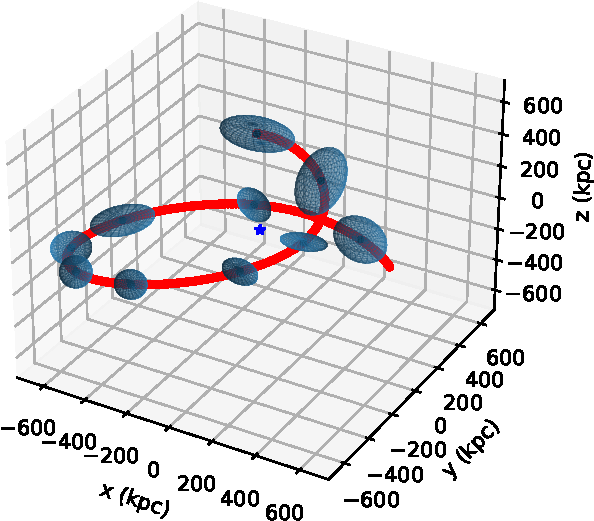
\includegraphics[width=\textwidth]{3d_qualitative_69p200.pdf}
\caption{Qualitative overview of the principal components ellipsoids for the stellar particle positions of the galaxy along its orbit.
In red the orbit of the galaxy (ID 69 with pericenter of 200 kpc).}
\label{fig:pca}
\end{figure}

\begin{figure}
\centering
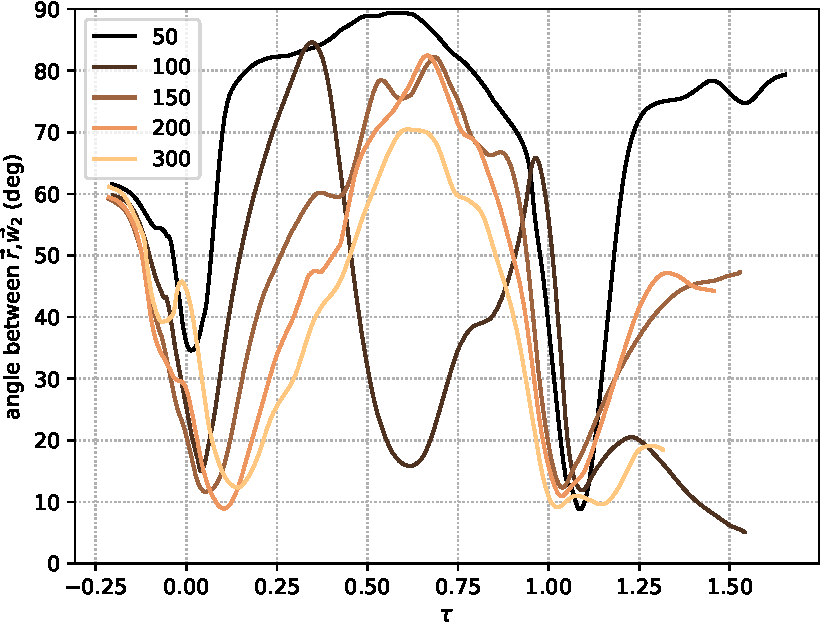
\includegraphics[width=0.8\textwidth]{69_r_angle.pdf}
\caption{Angle between the largest principal component $\vect{w}_2$ and the direction to the cluster center for simulation ID 69.}
\label{fig:pca_angle_r}
\end{figure}
\begin{figure}
\centering
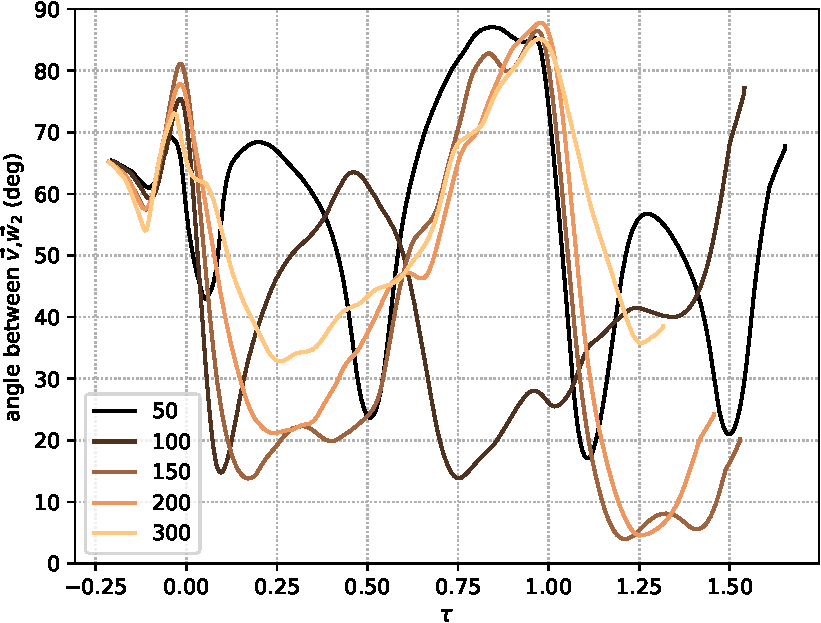
\includegraphics[width=0.8\textwidth]{69_v_angle.pdf}
\caption{Angle between the largest principal component $\vect{w}_2$ and the instantaneous velocity for simulation ID 69.}
\label{fig:pca_angle_v}
\end{figure}

\section{Star formation}
As shown in the previous section, elongation of material around low clustercentric distances may create grooves in the potential well which lead to angular-momentum transport.
In turn this helps funneling gas towards the center of the galaxy which is squeezed and can cool to create stars.
% TODO non gas run may isolate the role of star formation.
% Ram pressure stripping and tidal interaction can funnel gas into the inner part of the galaxy.
The total content of star forming gas is shown in cyan in Figure~\ref{fig:cold_gas} alongside with the specific star formation rate.
It is interesting to note that for an intermediate mass dwarf, the stripping phenomenon is highly nonlinear.
For example for simulation ID 68, as shown in the corresponding panel in Figure \ref{fig:cold_gas}, a slight change of orbit from 150~kpc pericenter to 100~kpc makes the dwarf completely stripped from the reservoir of cold gas.
Due to the stripping, after a burst, star formation stops.
\begin{figure}
\centering
\includegraphics[height=0.95\textheight]{{12.6_sfr_cold_gas}.pdf}
\caption{Specific star formation rate and cold gas (T<$15000$~K) evolution on different orbits.}
\label{fig:cold_gas}
\end{figure}

\citet{Tonnesen2012} argue that pressure in the cluster has a primary role in regulating SF as opposed to the strength of ram pressure.
% TODO Check: Also \citet{Hausammann2019} introduce the parameter $\beta$ defined as the ratio between the ram pressure and the thermal pressure as the

% TODO compute cluster gas pressure corresponding to SFR peaks.

\subsection{Where do stars form?}
\begin{figure*}
\centering
\begin{subfigure}[t]{0.74\textwidth}
\centering
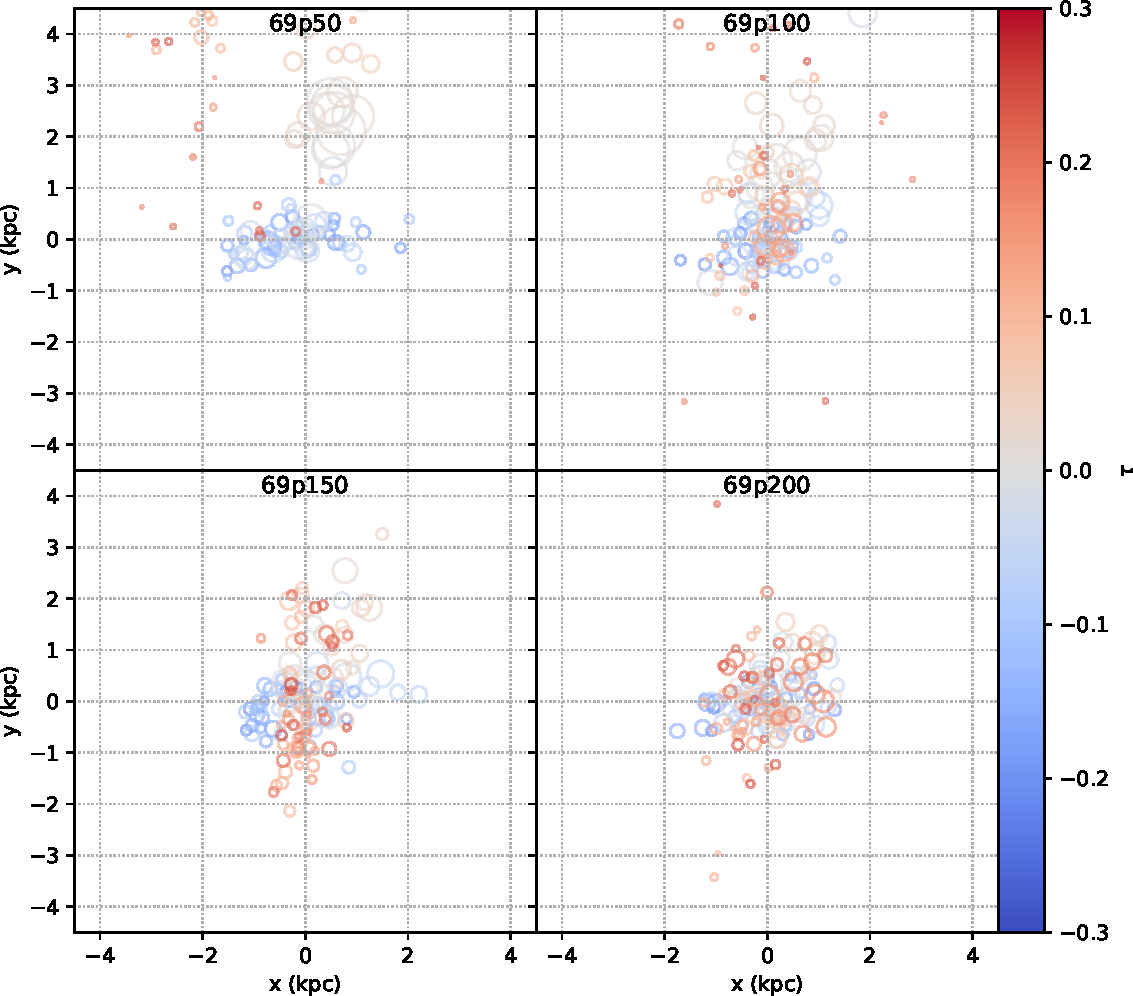
\includegraphics[width=\textwidth]{StarFormationLocation_new69_hollow.pdf}
\caption{Simulation ID 69}
\end{subfigure}\\[1.5ex]
\begin{subfigure}[t]{0.74\textwidth}
\centering
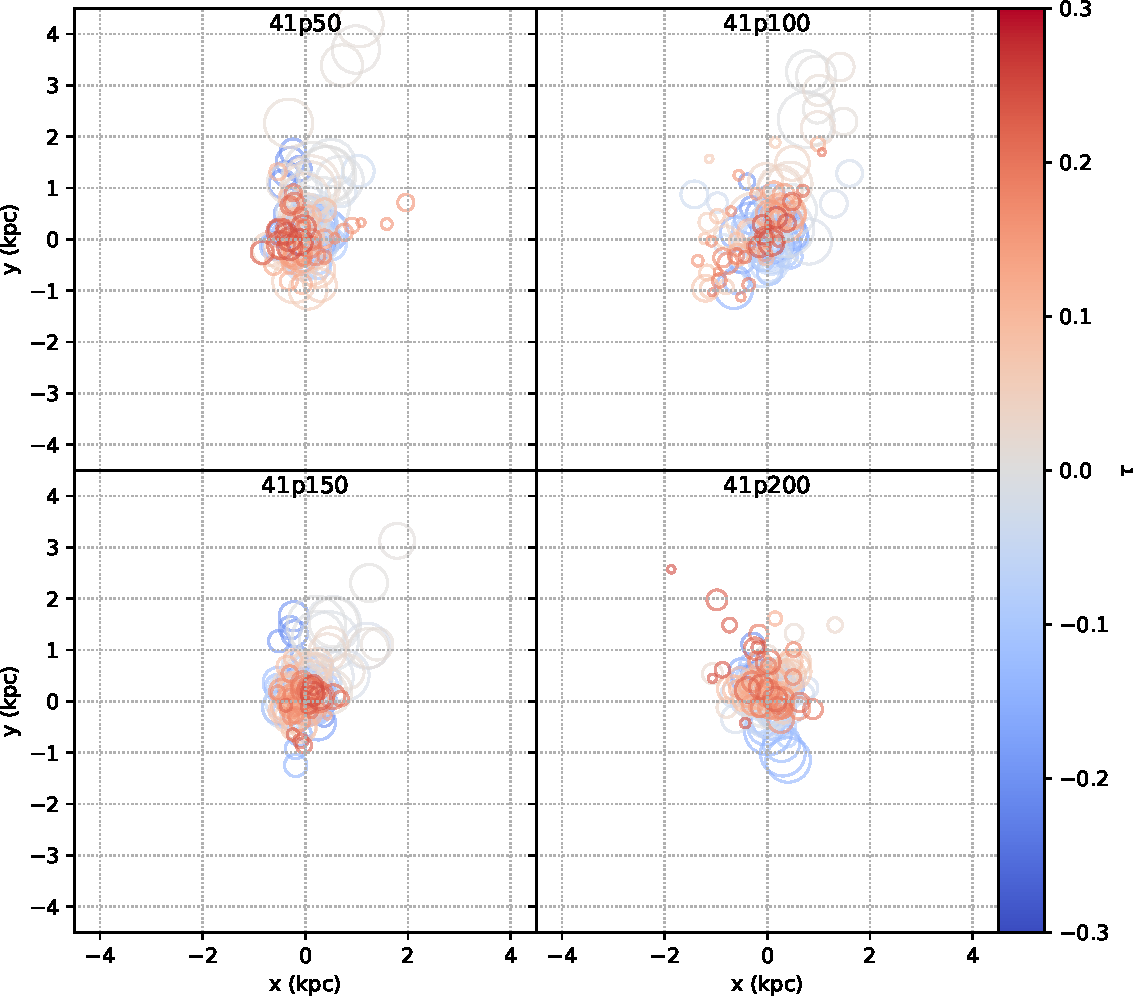
\includegraphics[width=\textwidth]{StarFormationLocation_new41_hollow.pdf}
\caption{Simulation ID 41}
\end{subfigure}
\caption{Star formation location around first pericenter passage for simulation ID 69 and~41.
Each subpanel corresponds to a different pericenter.
The size of the marker is proportional to the number of stars born in that time interval.
Markers are colored according to the time from pericenter normalized with the radial period.}
\label{fig:sf_location}
\end{figure*}
In Figure \ref{fig:sf_location} we show the average position of the star forming particles for each simulation snapshot.
The galaxy is moving in the $-y$ direction (the direction of the instantaneous velocity, see \refsec{sec:MovingBox}) around pericenter.
For each simulation snapshot the number of new stars w.r.t. to the previous snapshot ($10$~Myr before) is counted and their average position in the $xy$ plane is plotted.
\footnote{
We could have computed the star formation rate from the last galaxy snapshot at $z=0$, reading the time of formation of the star particles.
This is the common approach %\citep[e.g.][]{Hausammann2019}
when computing star formation histories of galaxies, and it is observationally motivated.
In fact the star formation history of an observed galaxy is inferred from the photometry and spectrum of the detected starlight.

However, the large amount of star particles lost during the orbit, leads to a large underestimation (of a maximum of 30\% for the most recent bins especially on low mass galaxies on radial orbits) of what has actually happened during the galaxy journey around the cluster.
The method of counting individual star particles newly born is therefore employed.
The choice of a high frequency snapshot cadence plays a fundamental role to this end.
}

In correspondence of pericenter passage an intense star formation activity is registered in the gaseous tail, see Figure~\ref{fig:sf_location}.
These galaxies can therefore be defined \emph{jellyfish} galaxies, when they are close to pericenter.
In stripped tails of the jellyfish, gas is able to cool and create stars.
This result supports the idea that the jellyfish phenomenon is a relatively short transitory phase of the galaxy along its orbit.

\section{Colour Magnitude} \label{sec:CM}
The catalogue of dwarf galaxies in the Fornax cluster, prepared by \citet{Venhola2019}, can be used to directly compare our results with observations.
We build the Color-Magnitude (C-M) diagram with all the simulation snapshots, after computing their SDSS-band colors and magnitude.
We then superimposed it on the results of the observations: as shown in Figure~\ref{fig:g-r} there is a good agreement between the catalogue values and our simulations.
In Fornax, the slopes of the C-M relations are different between the morphologically selected late-type and early-type galaxies.
The relation for the former is rather flat, meaning that the color is not correlated with magnitude, whereas the early-types become redder with increasing total luminosity.

In our simulations, the simulated dwarf galaxies tend to be blue and star-forming when they are near to the cluster center.
Tidal forces and ram-pressure boosts star formation, enhancing blue luminosities.
The initial mass of the galaxy plays an important role in defining how many times and for how long the galaxy moves between the late-type and early-type regimes.
In fact, if the galaxy gets stripped, it settles up on the early-type branch; if instead it can keep its gas, it turns blue again when falling into the cluster.
In particular the lightest galaxy (ID 62) does not survive the first infall yet ending its life in the early-type galaxy realm, independently of the orbit.
On the opposite end of the mass range, the most massive one (ID 41) retains most of its cold gas and, accordingly, its star formation occurs almost steadily, except for the most radial orbit.
Only for the 50 kpc orbit its final location on the C-M diagram is among the early-type galaxies.
Dwarfs on wide orbits, as shown in the 300~kpc pericenter panel of Figure~\ref{fig:g-r_sfr}}, stay on the blue branch indefinitely unless they become unbound (the condition \eqref{eq:tidal_radius_condition} ceases to be valid), as it happens for the low-mass galaxies.
Figure~\ref{fig:g-r_sfr} confirms that dwarfs rapidly turn red after quenching.

It is interesting to note that, for instance in the 50~kpc pericenter panel, dwarfs jump across the gap between the blue and red branches in between temporally equidistant snapshots.
Given that their color evolve rapidly, the gap between the two branches can be explained: an abundance of dwarfs is not expected in the color interval where their evolution is so quick.

% For the most massive galaxy instead star formation occurs almost steadily (\cf{} Figures~\ref{fig:g-r_sfr} and \ref{fig:cold_gas}).

\begin{sidewaysfigure}
\centering
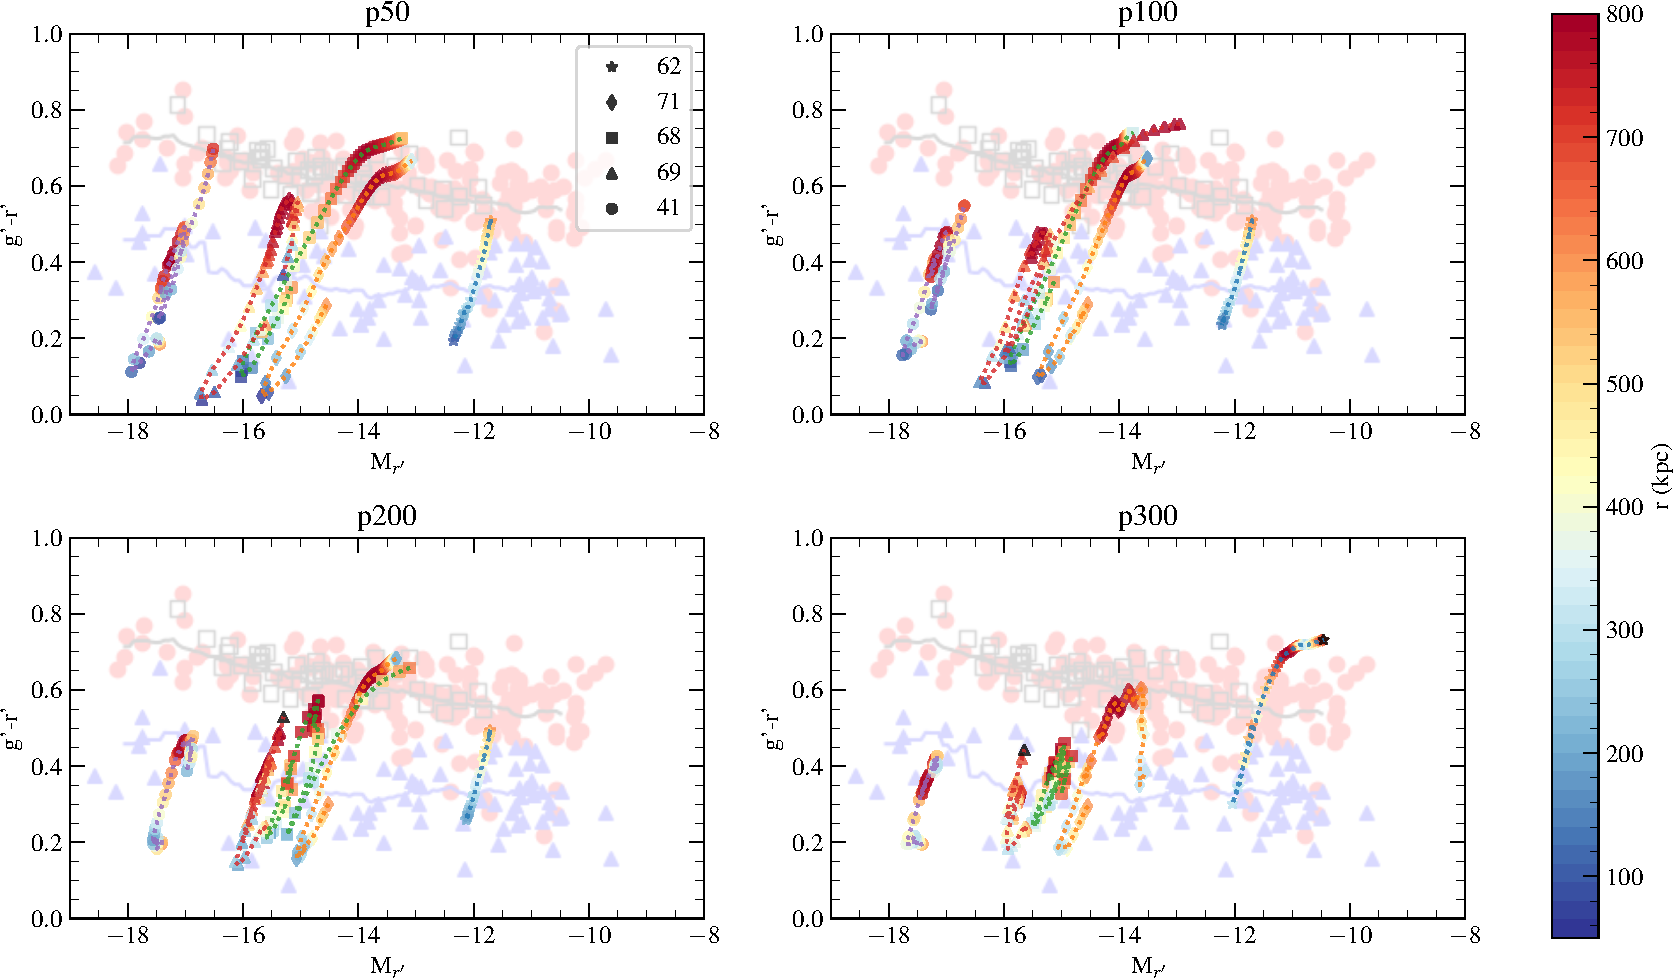
\includegraphics[width=\textwidth]{04.2_color_magnitude_Aku_g-r_rt_criterion_r.pdf}
\caption{SDSS bands colour magnitude diagram of galaxies on different orbits compared to Fornax dwarf catalogue of \citet{Venhola2019}.
% TODO ask permission for the overlay or use catalogue datapoints.
Red and blue colour for the data points in the background represent dwarf elliptical (dE) and late type galaxy respectively, classified by eye on the base of morphology.
Empty squares are nucleated dE.
Data tracks of simulated galaxies are shown overlaid colour coded by the clustercentric radius.
The tracks are limited to bound galaxies i.e. they are drawn with snapshots for which condition \eqref{eq:tidal_radius_condition} holds.
}
\label{fig:g-r}
\end{sidewaysfigure}
\begin{sidewaysfigure}
\centering
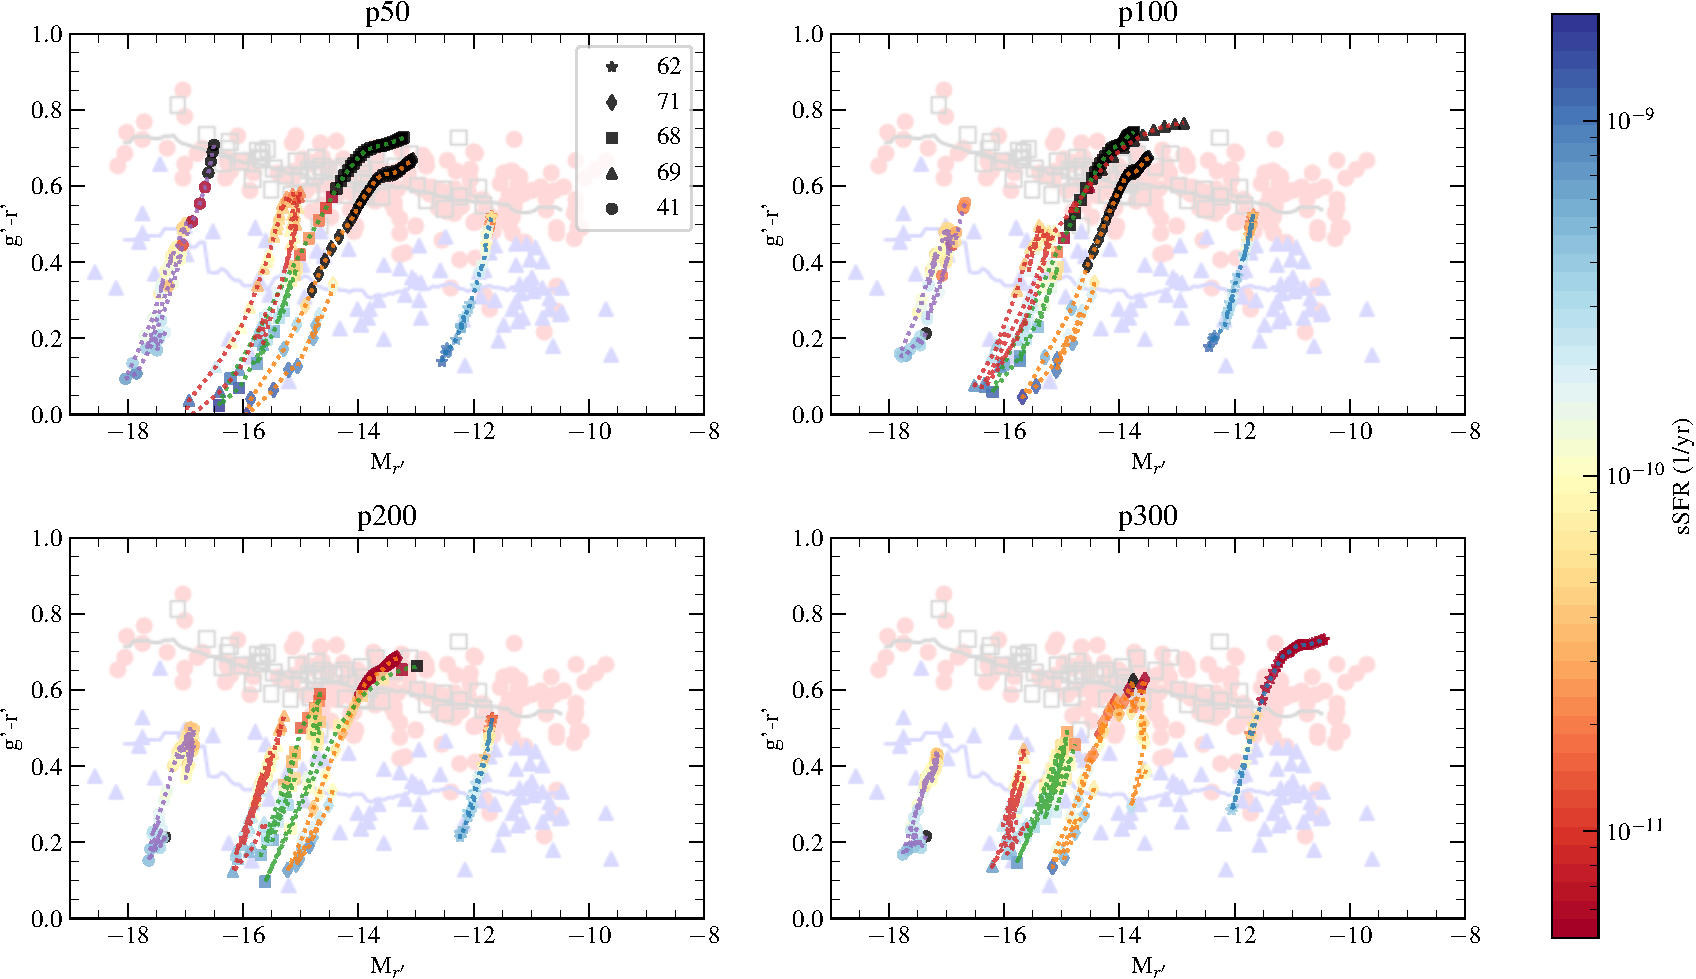
\includegraphics[width=\textwidth]{04.3_color_magnitude_Aku_g-r_rt_criterion_r_sfr.pdf}
\caption{Same as Figure~\ref{fig:g-r}, with point color coded with the specific star formation rate.
Black points are snapshots with no star formation.
}
\label{fig:g-r_sfr}
\end{sidewaysfigure}


\section{HI size mass relation during infall}
\citet{Stevens2019} show how inevitable is the size-mass relation of neutral hydrogen, even during stripping phases.
Our simulations can be checked on the size-mass plane.
As in \citet{Verbeke2017}, we computed the \Hi{} mass by integrating the \Hi{} column density $\Sigma_{\text{\Hi}}$. The radius on the other hand is the major axis of the best fit ellipse on the $1$~\Msun{}~pc$^{-2}$ contour.

%In Figure \ref{fig:hi_size_mass} we show the behaviour of the gas of a representative dwarf.
% We see that our dwarfs stay on the \Hi{} size-mass relation.

\section{Kinematics}
To correctly compute galaxy kinematics we have to take into account the rotation of the moving box.
The details on how to recover the correct kinematics in our setup are shown in \refsec{sec:correct_kinematics}.

\paragraph{Comparison with simulated galaxies in the field}
We compare the specific stellar angular momentum $j_s$ of particles within a sphere of $10$~kpc from the center of the galaxy both for a simulation in the moving box and for a run in isolation.
We notice in Figure \ref{fig:j_s_moria} an increase in angular momentum in correspondence to pericenter passages.

The combination of high velocity new stars and the gravitational energy injection given by the cluster at pericenter, result in a spin-up of the galaxy w.r.t. its evolution in the field.
% TODO metallicity gradient?

\begin{figure}
\centering
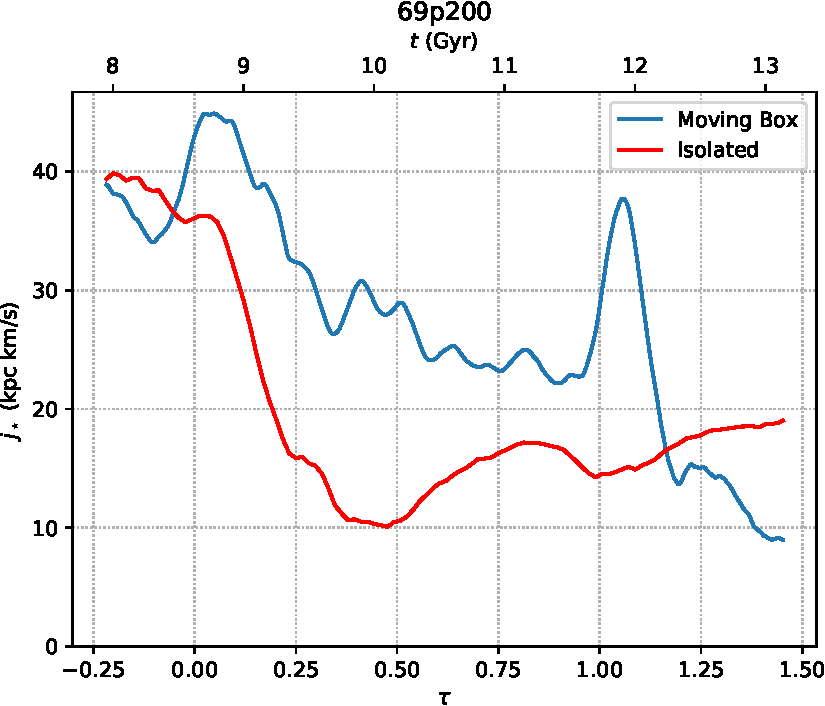
\includegraphics[width=0.6\textwidth]{15.0_angmom_inertial_moria.pdf}
\caption{Comparison between the norm of the specific angular momentum for the simulation ID 69 on a 200 kpc orbit and the correspondent isolated MoRIA run.}
\label{fig:j_s_moria}
\end{figure}

\subsection{Angular momentum and specific angular momentum proxy $\lambda_R$}
We compute the specific stellar angular momentum proxy $\lambda_R$ starting from SPH luminosity-weighted velocity and velocity dispersion maps as defined in \citet{Emsellem2007}: %\citet{Toloba2015}
\begin{equation}
 \lambda_R = \dfrac{\sum_i F_i R_i |V_i|}{\sum_i F_i R_i \sqrt{V_i^2 + \sigma_i^2}}
\end{equation}
with $i$ the pixel index, $F_i$ its flux and $R_i$ the distance of the pixel from the galaxy center.
This parameter has been introduced to better captures the spatial information included in the kinematic maps.
As opposed to the classical $\frac{v}{\sigma}$ indicator, $\lambda_R$ has been designed to distinguish between galaxies with kinematically decoupled components (KDC), which in some cases expose very similar $\frac{v}{\sigma}$.

An example of the maps from which $\lambda_R$ is computed for our simulation setup are shown in Figure~\ref{fig:maps_lambda_r}.
The $V_{LOS}$ and $\sigma$ map are computed with SPH interpolation, using the luminosity in $v$-band to weight the contribution of particles along the line of sight.
Some authors \citep[e.g.][]{Schulze2018,Pillepich2019} use non-weighted quantities taken directly from the particles to compare simulations and observation.%, even if what is observed are luminosity-weighted measures.
This approach makes the comparison with observations more difficult since all the information that we get is luminosity weighted \citep{Walo-Martin2020}.

\begin{figure}
\centering
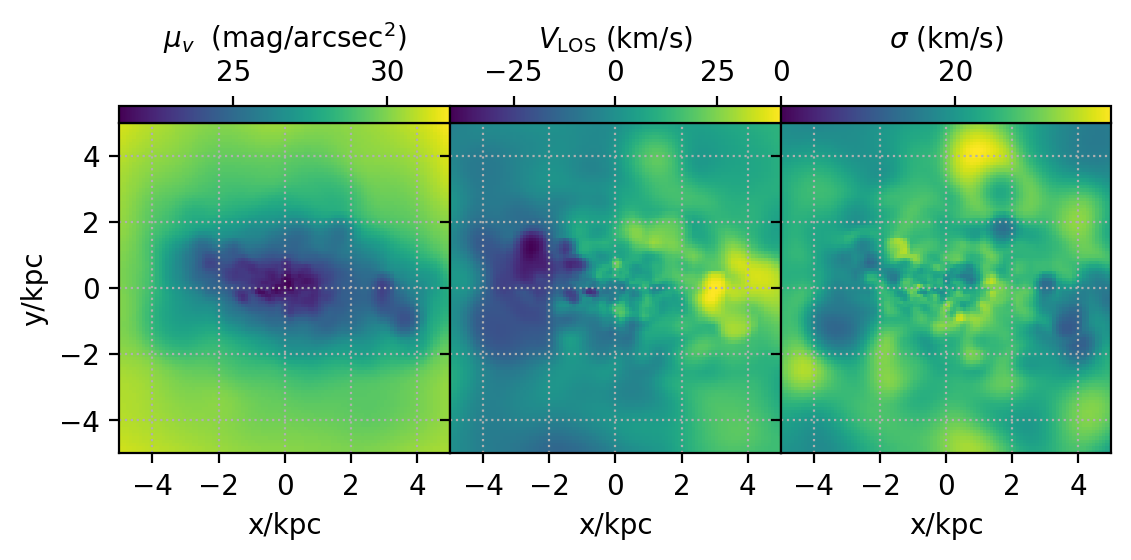
\includegraphics[width=\textwidth]{mu_v_sigma_69p150s60_sideon.png}
\caption{$\mu_v$ surface brightness map and SPH v-band luminosity weighted maps of line of sight velocity and velocity dispersion $\sigma$ for a snapshot of the simulation ID 69 around first pericenter passagethatthat.
The galaxy is projected edge-on, with the angular momentum vector lying on the $xy$ plane.}
\label{fig:maps_lambda_r}
\end{figure}

\begin{figure}
\centering
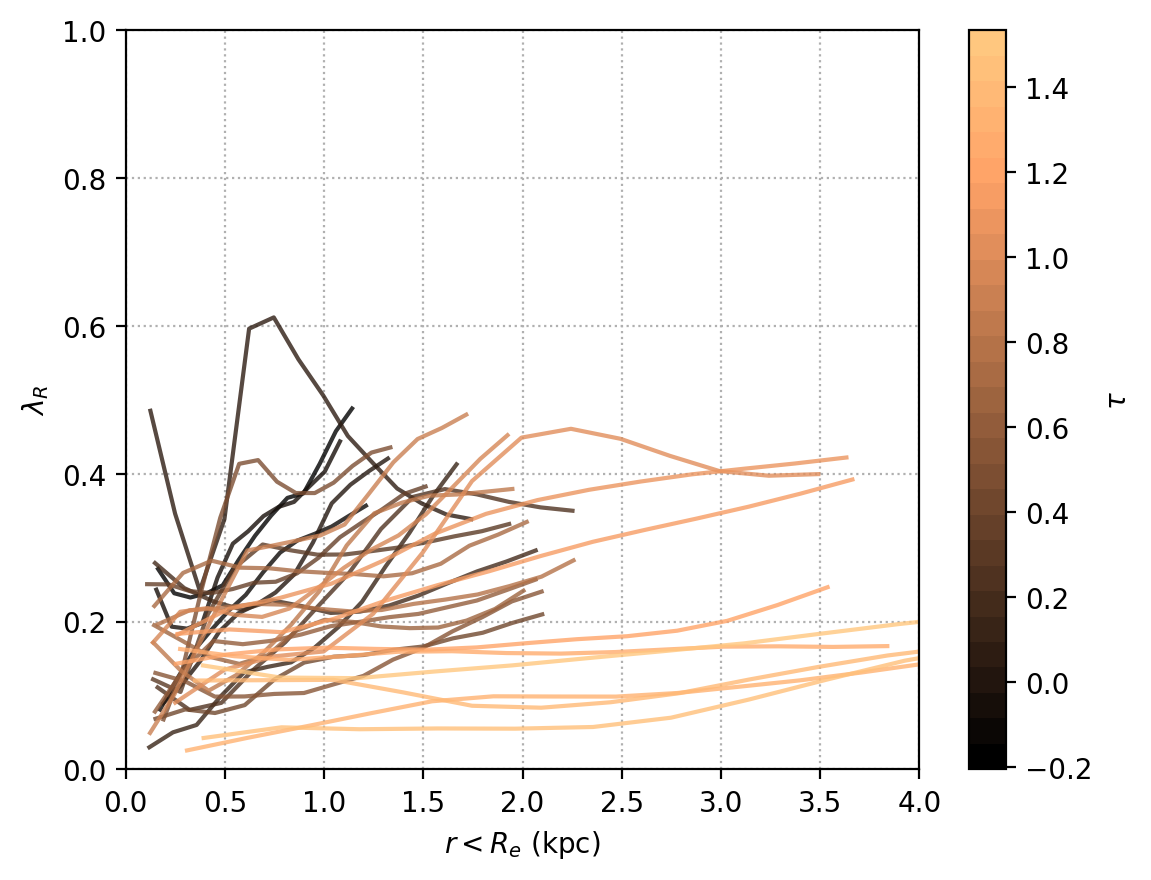
\includegraphics[height=0.42\textheight]{lambda_r_profile_69p150_each20_up_to_r_e.png}
\caption{$\lambda_R$ profiles for ID 69 on a 150 kpc orbit color coded with time normalized by radial period. The $\lambda_R$ profile is show up to the corresponding $R_e$.}
\label{fig:lambda_r_profile}
\end{figure}

It is possible to compute the radial profile of $\lambda_R(r)$, as in Figure~\ref{fig:lambda_r_profile}.
The profile itself and the value $\lambda_R(R_e) = \lambda_{R_e}$ is used to distinguish between fast and slow rotators.
\citet{Emsellem2007} defines galaxies with $\lambda_R < 0.1$ as ``slow rotators'' whereas the one with $\lambda_R>0.1$ as ``fast rotators''.
As shown in Figure~\ref{fig:lambda_r_profile}, galaxies while falling into the cluster, evolve from being classified as having a fast rotators profile to slow rotator \citep[cf.][]{Emsellem2011}.

% Obviously this distinction depends on the real inclination of the galaxy, as it appears in the sky. % TODO possible to include inclination in a plot?

It has been shown in the \textsc{SMAKCED} survey of 39 early-type galaxies in the Virgo cluster \citep{Toloba2014, Toloba2015} that the so classified fast-rotator galaxies in the outer region of the cluster rotate faster than the fast rotators in the center of the cluster.
The observed specific angular momentum $\lambda_R$ is correlated with clustercentric distance. % FIXME \citep{Bidaran2020}. citep DEugenio2015
It is indeed hypothesized, that after pericenter passages and a long time in the cluster, galaxies are heated up and transformed into slow rotating dEs.
This scenario is confirmed by our simulations where dwarf irregulars are converted to early-type galaxies and as time (normalize with radial period $\tau$, as in Figure~\ref{fig:lambda_r_profile}) their kinematics is transformed into the one of slow rotators.

In our case, however, the correlation of $\lambda_R$ with clustercentric distance is mild and affected by the very noisy and time-dependent nature of the angular momentum proxy.
For example in simulation ID 69, as shown in Figure~\ref{fig:lambda_r_j_s}, $\lambda_R$ behaviour is very oscillating and quite prone to bursty star formation which can abruptly affect its value.
In our measurements, $\lambda_R$ fails to distinguish pericenter passages unequivocally.

\begin{figure}
\centering
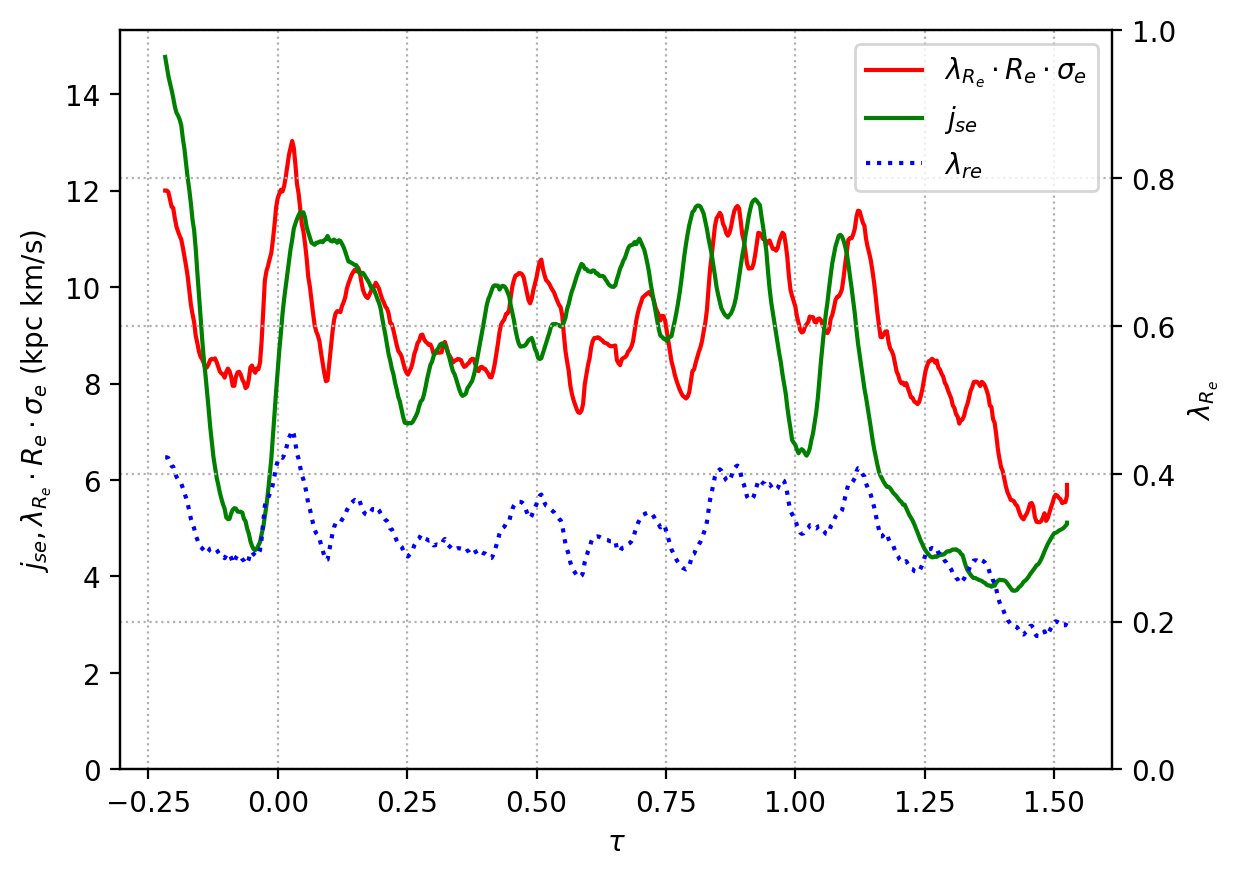
\includegraphics[height=0.42\textheight]{lambda_r_j_s_69p150r100.png}
\caption{Comparison between specific angular momentum and $\lambda_R$ at the effective radius for ID 69 on a 150 kpc orbit.
$\lambda_R$ is computed viewing the galaxy side-on.
Curves are smoothed using a rolling average of 0.2~Gyr.}
\label{fig:lambda_r_j_s_sigma}
\end{figure}

\begin{figure}
\centering
\includegraphics[height=0.9\textheight]{{02.1_lambda_r_vs_js}.pdf}
\caption{Stellar specific angular momentum proxy $\lambda_R$ and specific angular momentum of star particles $j_s$ for the simulation ID 69 on multiple orbits. The measurements have been taken by observing he galaxy from the plane of the orbit, recreating the condition of a fixed observer.}
\label{fig:lambda_r_j_s}
\end{figure}

% TODO The relative increase of $\lambda_R$ at first pericenter passage is shown for each orbit and mass in figure \ref{fig:ssam_relative}.
% Around pericenter passages an increase of $\lambda_R$ by a factor of $\approx 2$ is observed.

% 

\subsection{Relation between $\lambda_R$ and physical angular momentum TO BE FINISHED}
% We wanted to 
First we compute the specific angular momentum $\vect{j}_{s}$ of star particles within $10$~kpc from the center of the galaxy.
\begin{equation}
\vect{j}_{se} = \sum_{i\in S} \vect{r}_i\cross\vect{v}_i,\quad \text{where } S\equiv\{k: \norm{\vect{r}_k} < R_e.\} 
\end{equation}
% We compute the specific angular momentum $\vect{j}_s$ of star particles within 10~kpc from the center of the galaxy (densest stellar region):
% \begin{equation}
% \vect{j}_s = \sum_{i\in S} \vect{r}_i\cross\vect{v}_i,\quad \text{where } S\equiv\{k: \norm{\vect{r}_k} < 10 \text{~kpc.}\} 
% \end{equation}
% ($\vect{j}_s = \vect{J}_s/M_\star$ where $J_s$ is the total angular momentum and $M_\star$ the stellar mass of the galaxy)
% We compare $\vect{j}_{s}$ with $\lambda_R$ in Figure \ref{fig:lambda_r_j_s}.


\paragraph{Comparing $j_{se}$ with observables} We tried to retrieve the In order to compare the proxy $\lambda_R$ with the angular momentum, we try to retrieve an approximate formula for the specific angular momentum which relies on observable quantities:
\begin{equation}
 j_s^* = \lambda_R \cdot R_e \cdot \sigma_e 
\end{equation}
where $\sigma_e$ is the line-of-sight velocity dispersion of star particles measured within an aperture of $R_e$.
% This formula reasonably reintroduces physical dependency.

% We shall see that.
% Another effect is at play: maps as those in Figure~\ref{fig:maps_lambda_r} show
% For simplicity this 

The relation between $\lambda_R$ and $j_s^*$ is shown in Figure~\ref{fig:lambda_r_j_s_sigma}

%As also found by, ... we confirm that it is very sensitive to recent episode of star formation, especially the ones due to gas stripping, where young stars are 
% For these reasons in the case of dwarf irregulars it is not a good indicator of the real rotation of the galaxy.
% TODO 41 69 71
% 
% \begin{figure}
% \centering
% 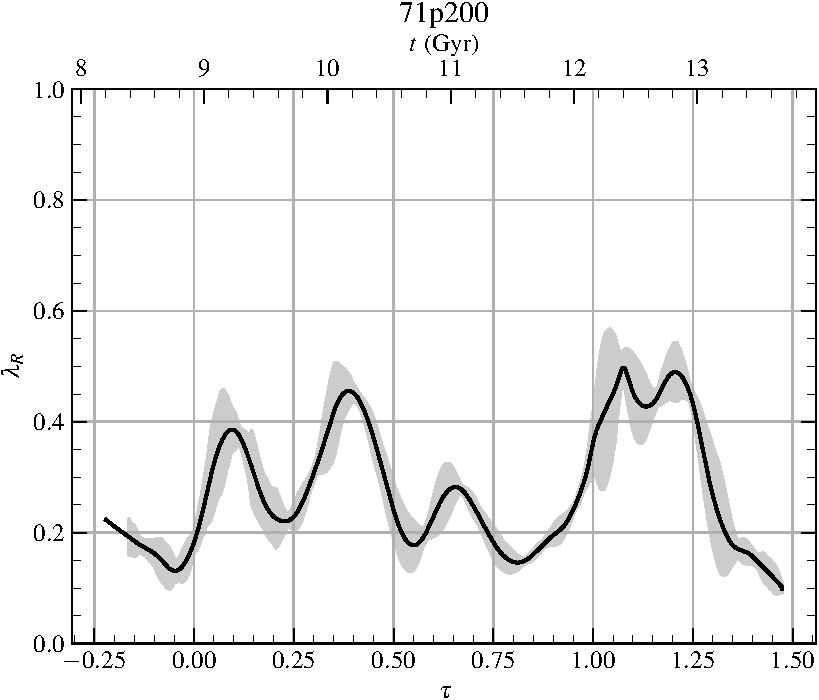
\includegraphics[width=.8\columnwidth]{03.0_fig_lambda_r_time.pdf}
% \caption{Specific stellar angular momentum for galaxy ID 71 on a $200$~kpc pericenter orbit.}
% \label{fig:lambda_R}
% \end{figure}

\section{Conclusion}

\begin{itemize}
 \item $\lambda_R$ is very variable with time in the dwarf irregular regime.
 \item It is sensitive to many things. % FIXME
 \item There can be cases in which depending on the projection and the size of the galaxy, $\lambda_R$ correlates poorly with the physical specific angular momentum.
\end{itemize}


% \subsection{Magnitude conversion}
% \pynbody{} can be programmed to compute luminosities of stellar particles using 
% The built in libraries are from Marico... Padova... %TODO
% To obtain SDSS bands we ued conversion formulas from here, after having computed the magnitudes in Johnson bands.
% 
% In particular:

